\chapter{Results and Interpretation}
\label{chap:results}

The background estimation techniques described in the previous chapters are used to make predictions
in each of the 282 signal regions bins. We then compare and fit to observed event counts, using a
maximum-likelihood fit that takes into account all statistical and systematic uncertainties.
Finally, the results of this fit are used to constrain a variety of beyond-the-standard-model physics
scenarios. Sec.~\ref{sec:prefit} presents the raw, pre-fit results, Sec.~\ref{sec:fits} briefly describes
the fitting and limit-setting procedures, and Secs.~\ref{sec:susy_interp} and \ref{sec:lq_interp} show 
the resulting limits placed on all considered signal models.

\section{Pre-fit results}
\label{sec:prefit}

Figures~\ref{fig:results_mono_vl} to \ref{fig:results_incl} show comparisons of the pre-fit background estimates
and observed yields in all signal regions. The hatched regions in the upper panels (and the solid gray bands
in the ratio panels) represent the total statistical and systematic uncertainty in the background prediction.
For the monojet region, the $x$ axis binning is $\pt^\mrm{jet1}$ (in\GeV), and for the $\Nj\geq2$ regions
the $x$ axis binning is \mttwo (in\GeV). Dashed lines separate the bins into categories of \Nj and \Nb.
Observed yields are statistically consistent with the estimated SM background.

\begin{figure}[htbp]
  \begin{center}
    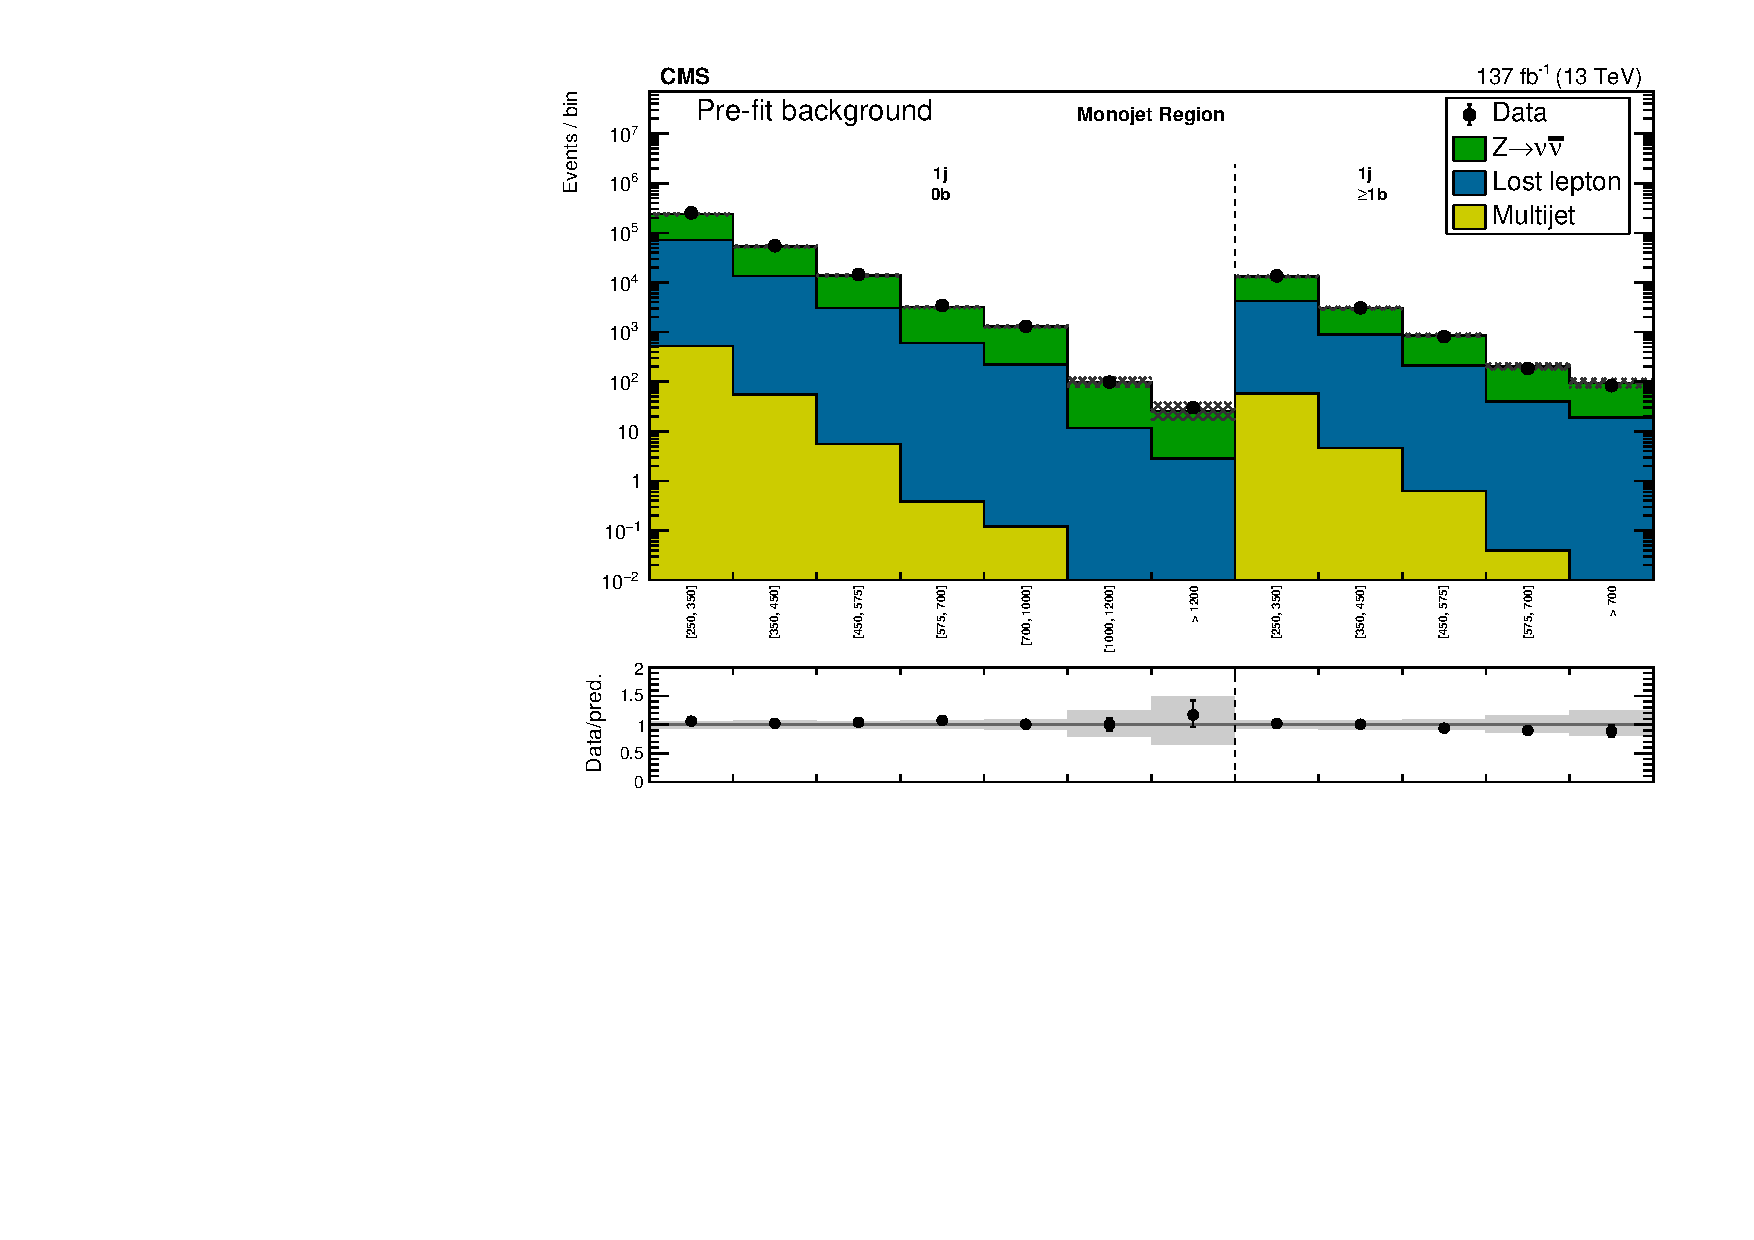
\includegraphics[width=0.93\textwidth]{figs/results/prefit_monojet_ratio.pdf} \\
    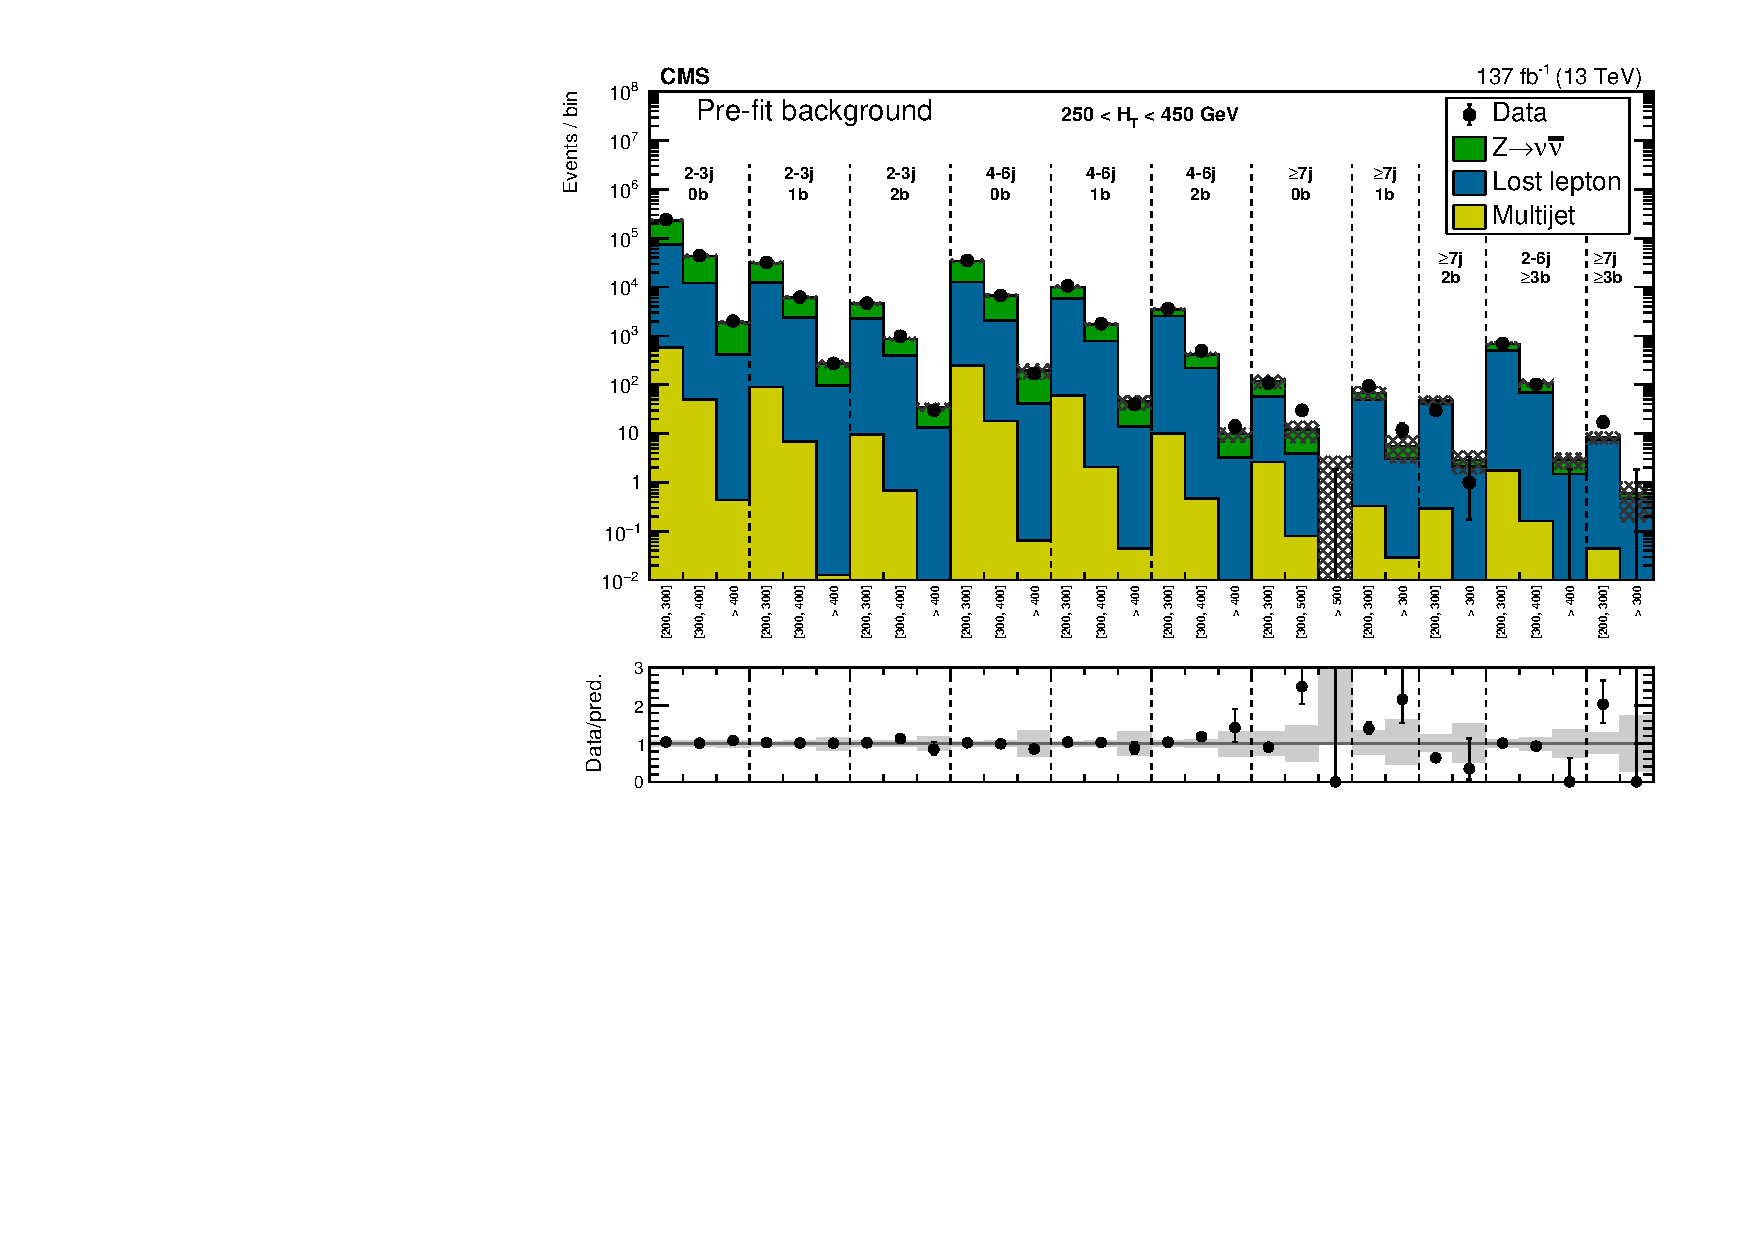
\includegraphics[width=0.93\textwidth]{figs/results/prefit_HT250to450_ratio.pdf} \\
    \caption{Expected (pre-fit) and observed yields for the full dataset collected from
      2016--18, corresponding to an integrated luminosity of \Lint. On top are the monojet
      signal regions, separated into \Nb categories and with $\pt^\mrm{jet1}$ binning on the $x$ axis.
      On the bottom are the $\Nj\geq2$ signal regions with $250 \leq \Ht < 450\GeV$, separated into
      topological regions with the \mttwo binning on the $x$ axis.
            }
    \label{fig:results_mono_vl}
  \end{center}
\end{figure}

\begin{figure}[htbp]
  \begin{center}
    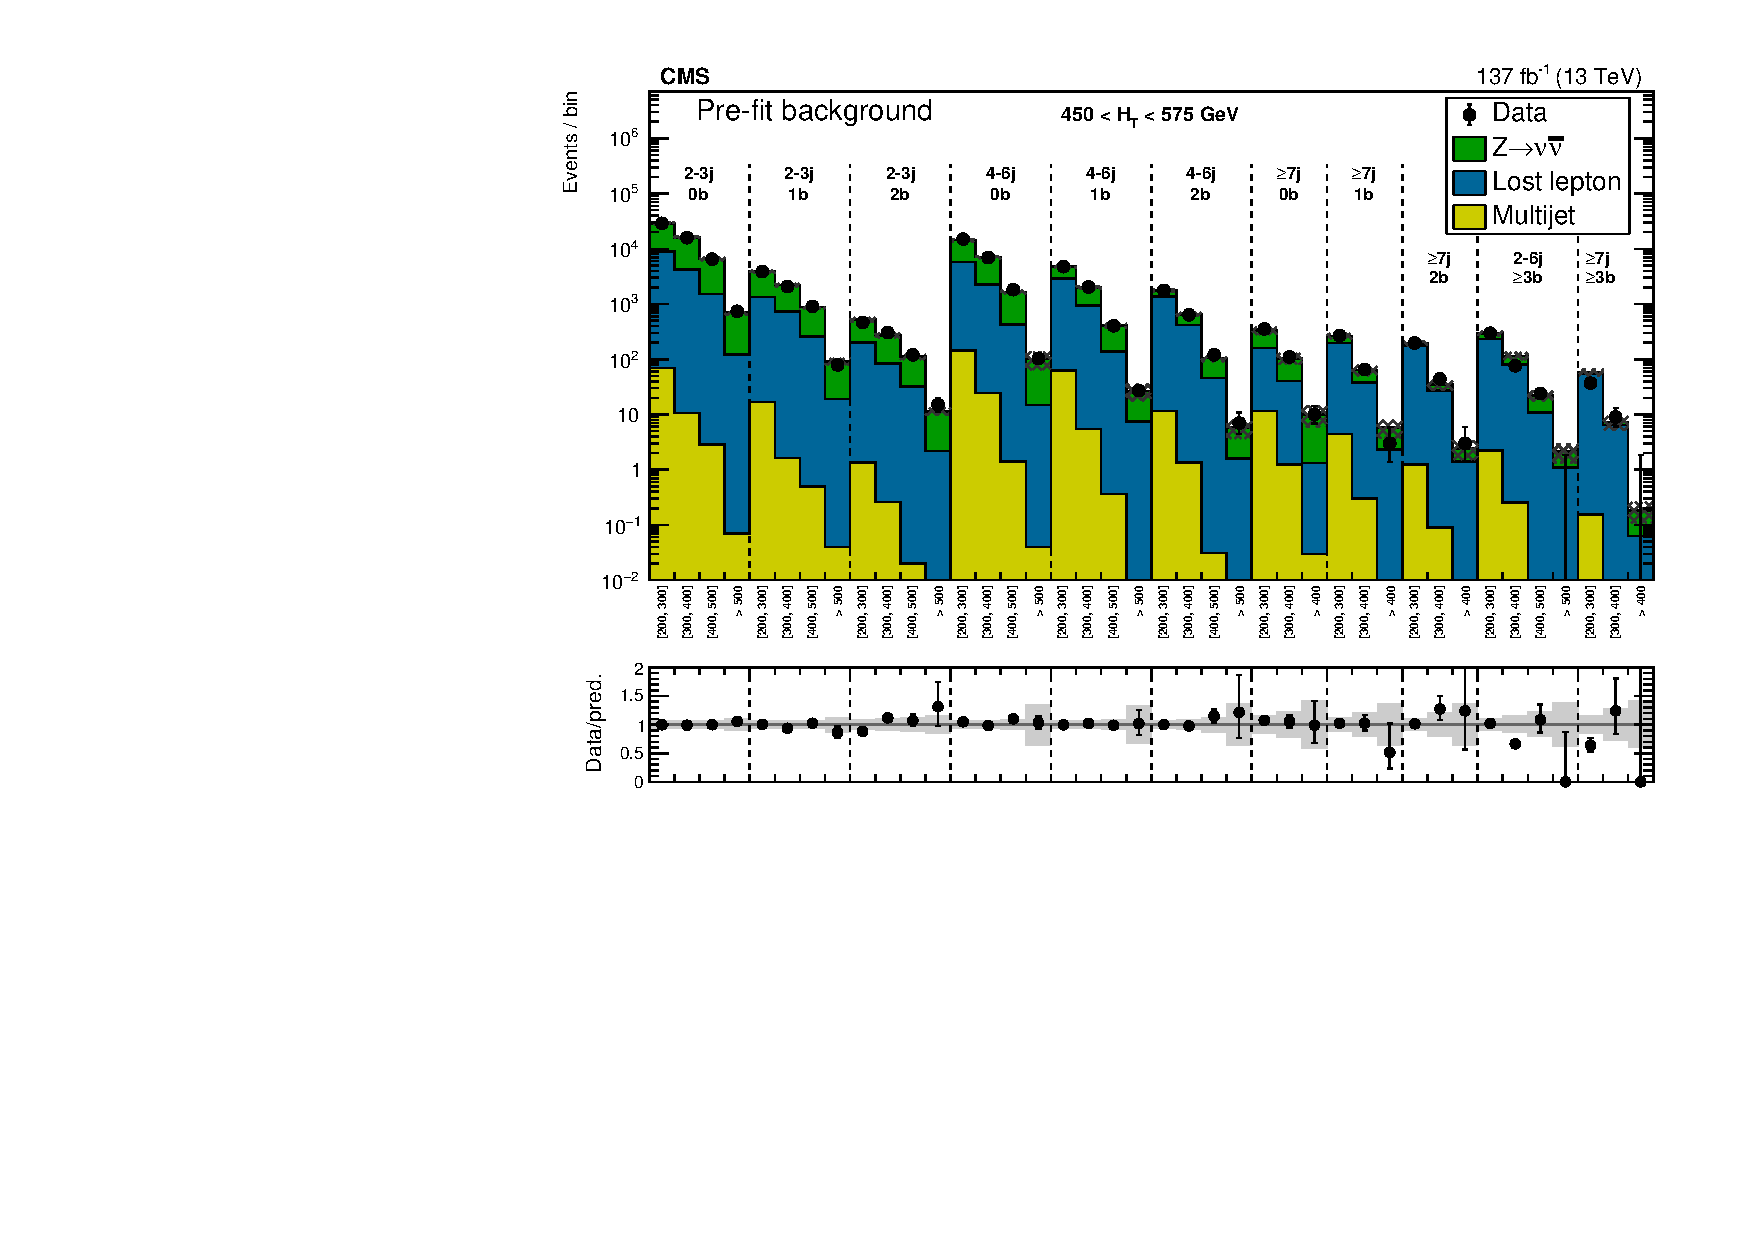
\includegraphics[width=0.93\textwidth]{figs/results/prefit_HT450to575_ratio.pdf} \\
    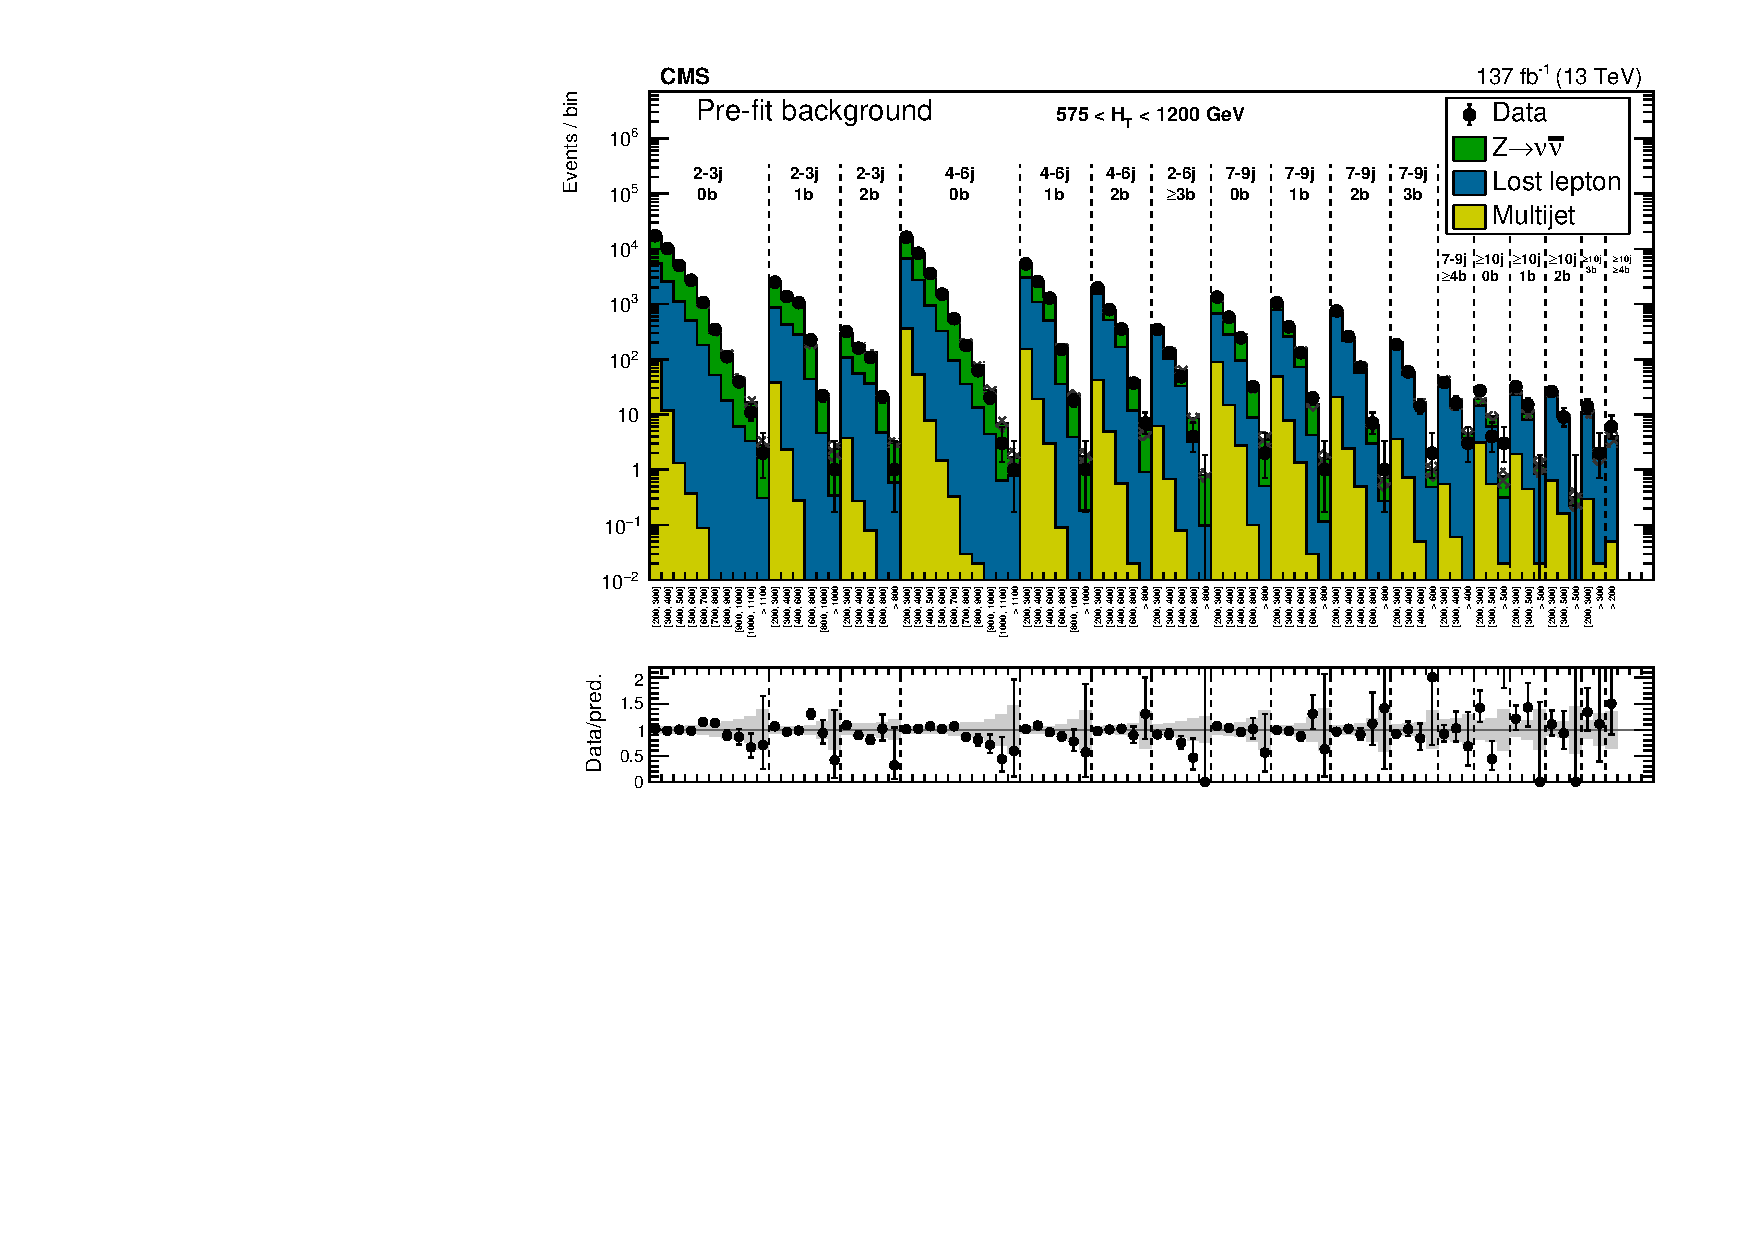
\includegraphics[width=0.93\textwidth]{figs/results/prefit_HT575to1200_ratio.pdf} \\
    \caption{Expected (pre-fit) and observed yields for the full dataset collected from
      2016--18, corresponding to an integrated luminosity of \Lint. The top and bottom figures
      contain the $\Nj\geq2$ signal regions for the $450 \leq \Ht < 575\GeV$ and $575 \leq \Ht < 1200\GeV$
      regions, respectively. \mttwo binning is shown on the $x$ axis, with the dashed lines separating
      bins by topological region.
            }
    \label{fig:results_l_m}
  \end{center}
\end{figure}

\begin{figure}[htbp]
  \begin{center}
    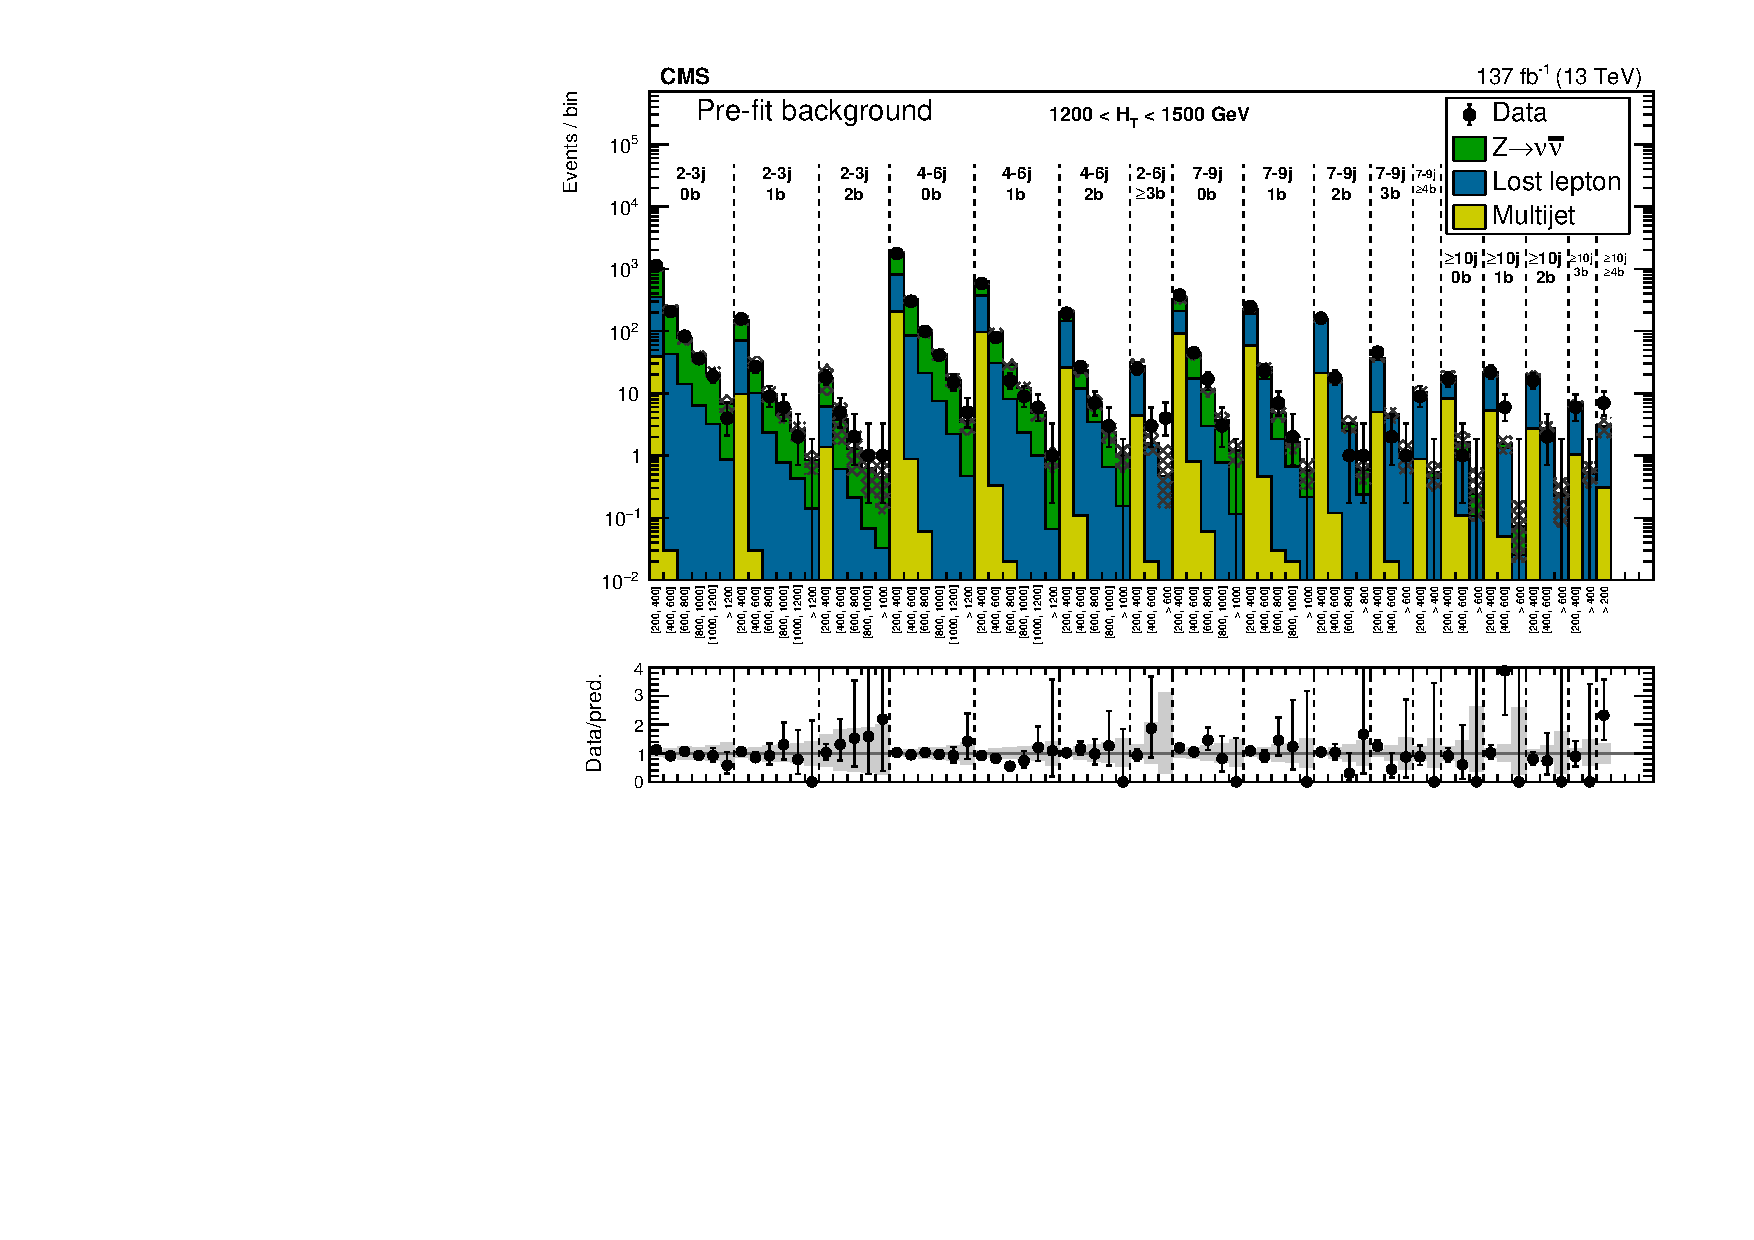
\includegraphics[width=0.93\textwidth]{figs/results/prefit_HT1200to1500_ratio.pdf} \\
    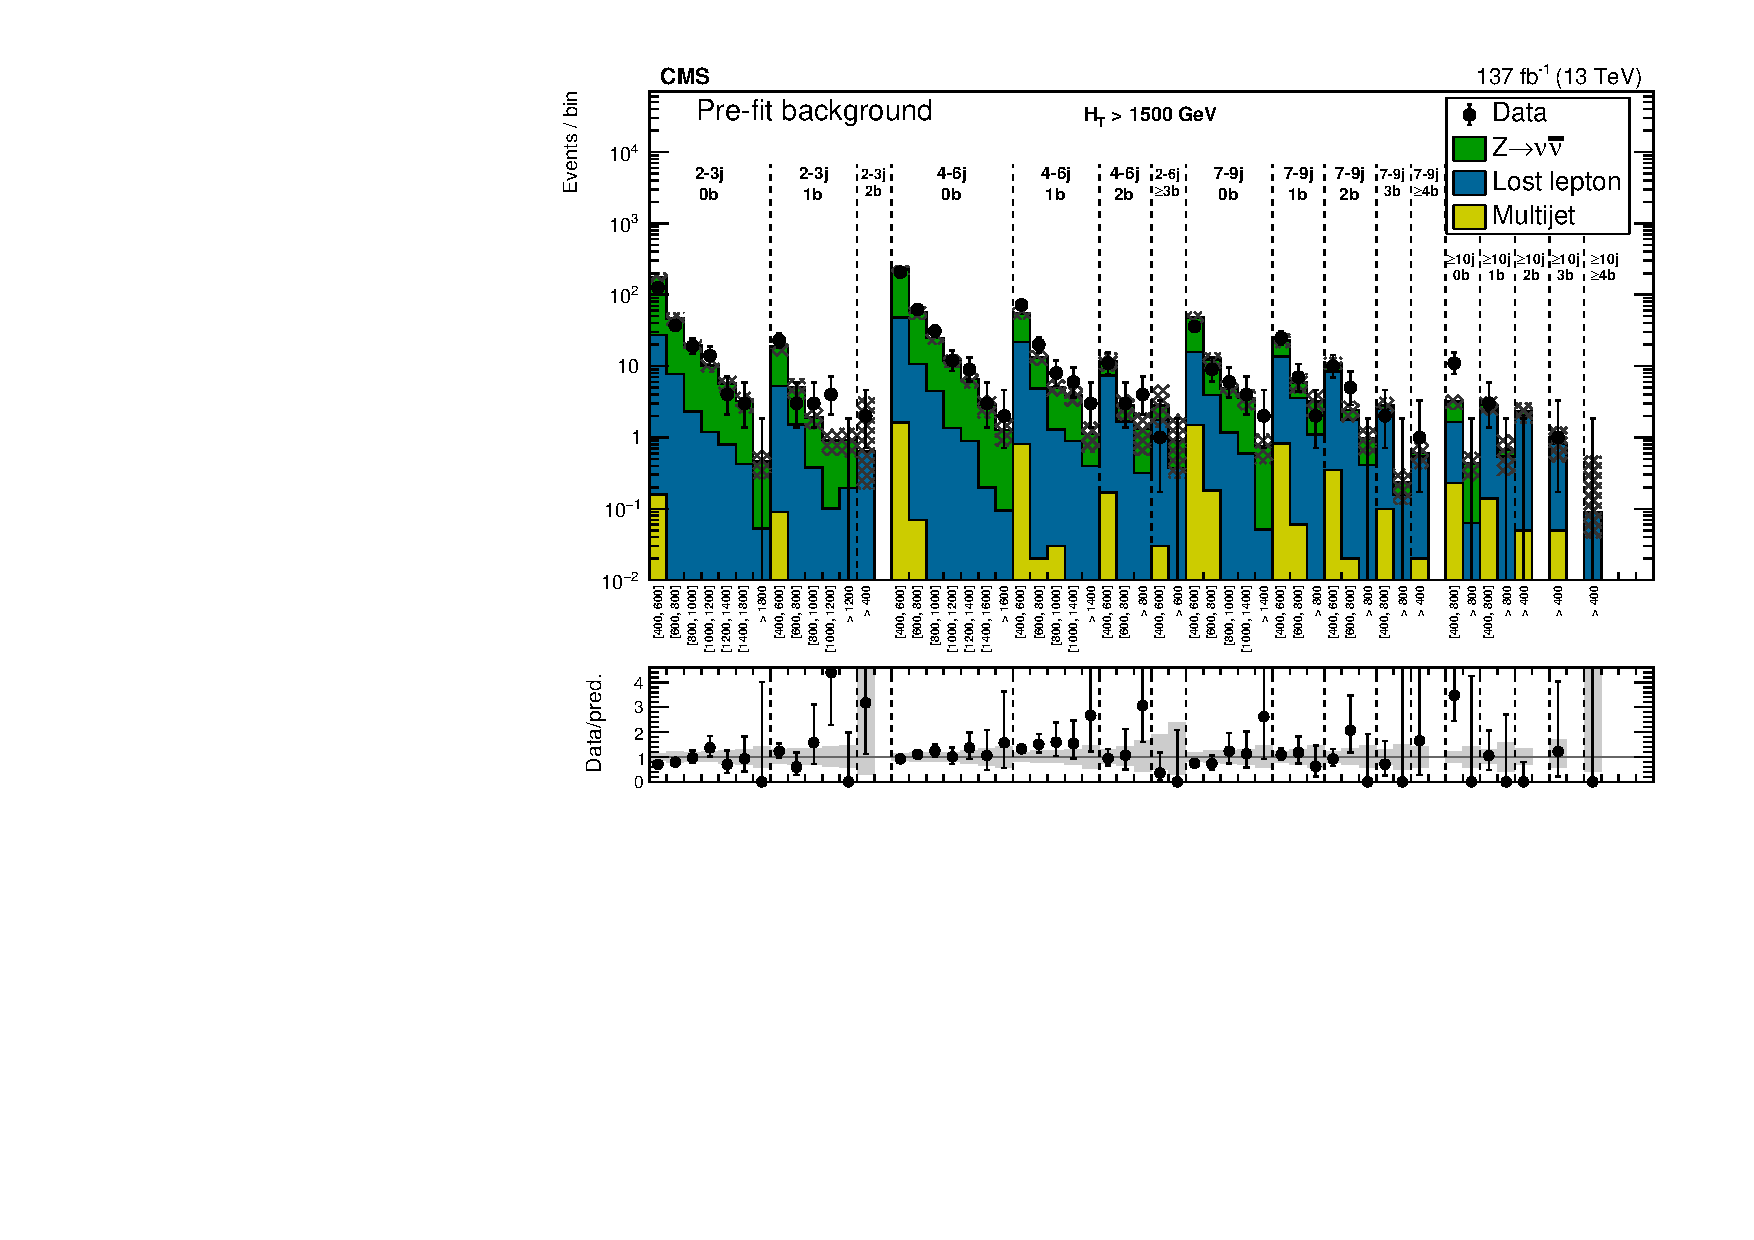
\includegraphics[width=0.93\textwidth]{figs/results/prefit_HT1500toInf_ratio.pdf} \\
    \caption{Expected (pre-fit) and observed yields for the full dataset collected from
      2016--18, corresponding to an integrated luminosity of \Lint. The top and bottom figures
      contain the $\Nj\geq2$ signal regions for the $1200 \leq \Ht < 1500\GeV$ and $\Ht\geq1500\GeV$
      regions, respectively. \mttwo binning is shown on the $x$ axis, with the dashed lines separating
      bins by topological region.
            }
    \label{fig:results_h_uh}
  \end{center}
\end{figure}

\begin{figure}[htbp]
  \begin{center}
    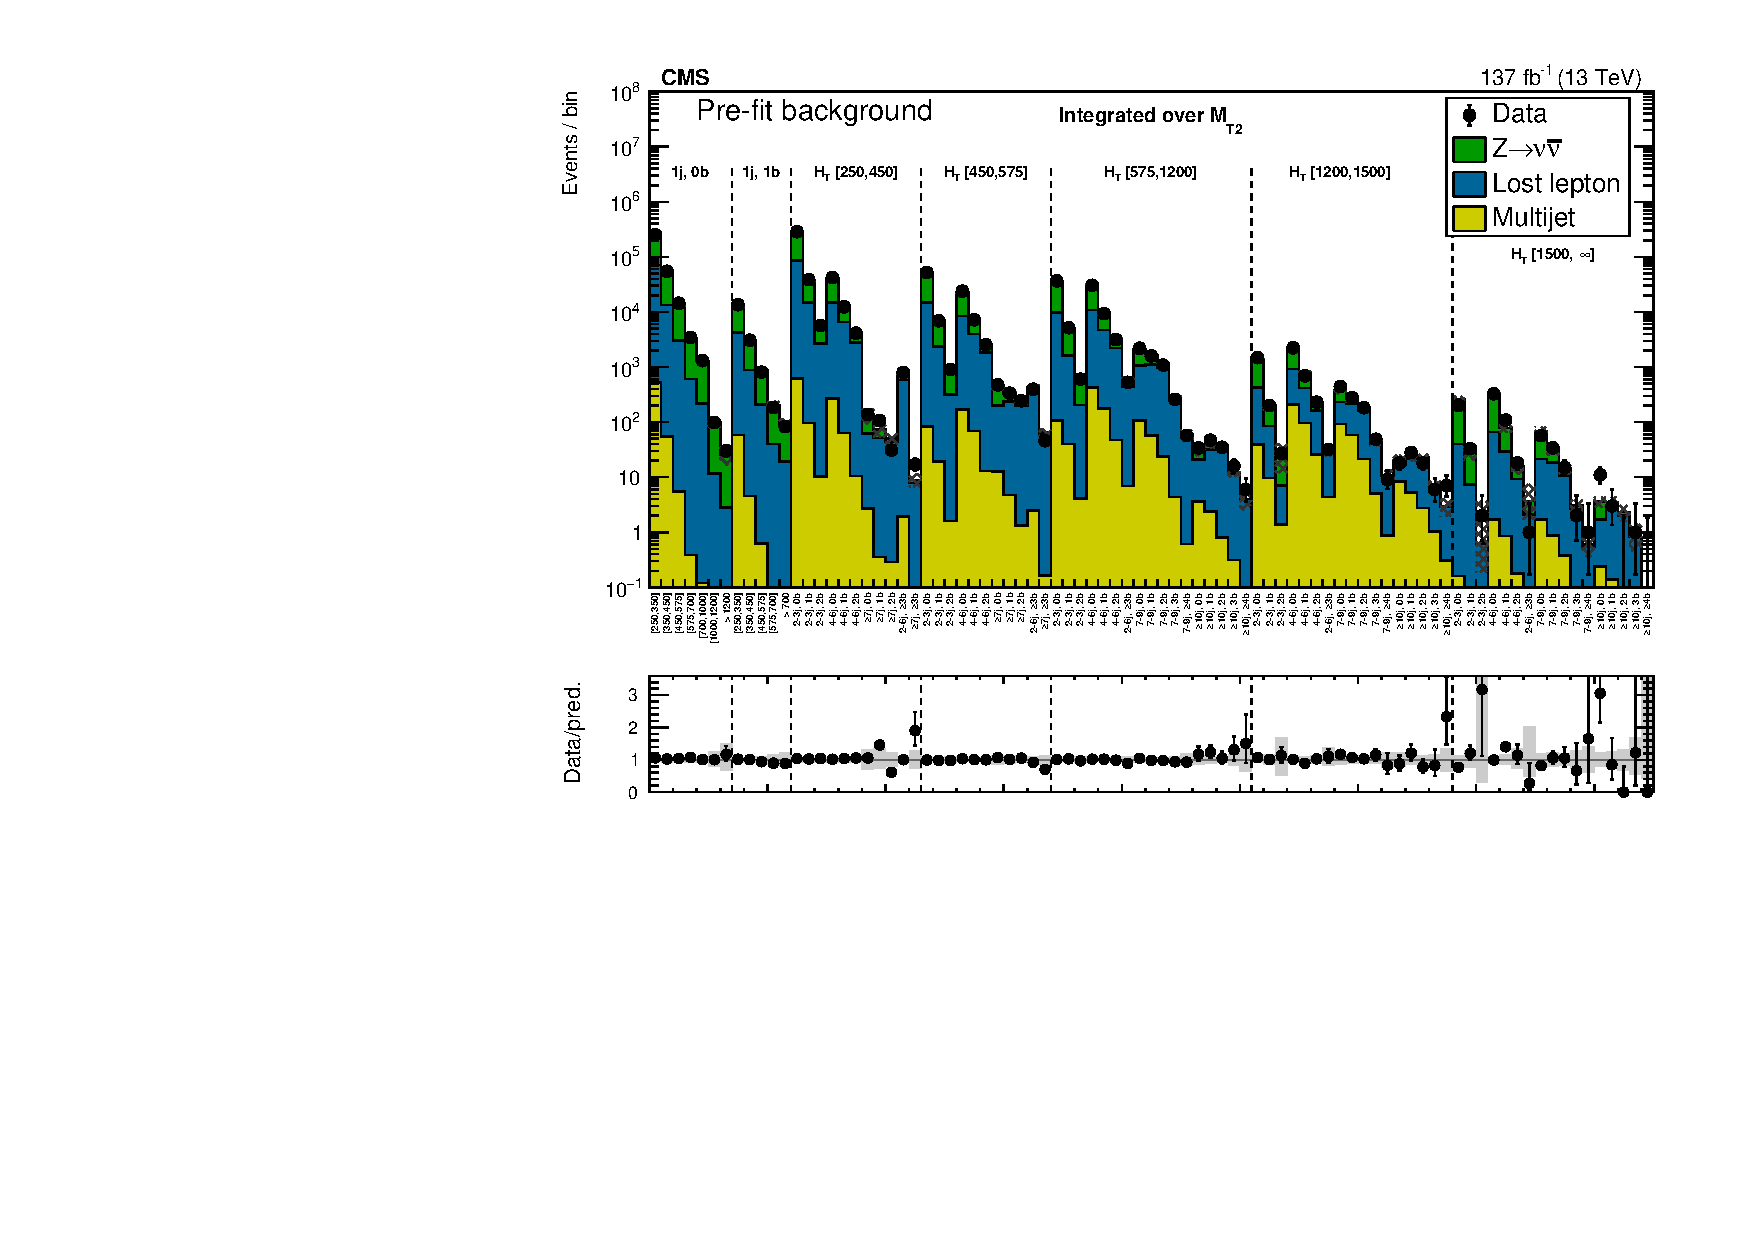
\includegraphics[width=0.93\textwidth]{figs/results/prefit_inclusive.pdf}
    \caption{Expected (pre-fit) and observed yields for the full dataset collected from
      2016--18, corresponding to an integrated luminosity of \Lint. Here the results are shown
      integrated over \mttwo, with each bin on the $x$ axis corresponding to an \Nj/\Nb topological
      region. Dashed lines separate the various \Ht regions. The two leftmost regions contain the monojet
      signal regions, where the $x$ axis binning is $\pt^\mrm{jet1}$.
            }
    \label{fig:results_incl}
  \end{center}
\end{figure}


\section{Maximum-likelihood fits and the \texorpdfstring{CL$_\text{S}$}{CLs} technique}
\label{sec:fits}

The results presented in the previous section are \textit{pre-fit}, meaning the shown backgrounds
and uncertainties are straight from the estimation methods, without attempting to fit to the data
in any way. For the purposes of evaluating the results and setting constraints on models of new physics,
we apply a fitting procedure to test the compatibility of the observed results with SM predictions.

The expected background and signal yields are functions of \textit{nuisance parameters}, which represent
the potential variations from all of the experimental and theoretical uncertainties. In practice these
are modeled as log-normal constraints on the background and signal yields (except for statistical uncertainties
on the observed control region event counts, which are modeled as gamma functions). Denoting the vector
of all nuisance parameters as $\theta$, and their joint probability distribution as $p(\theta)$, we can write
the complete likelihood function as
\be
\mathcal{L}(\mrm{data}|\mu,\theta) = \prod_{j\in\mrm{bins}} \frac{[\mu s_j(\theta)+b_j(\theta)]^{n_j}}{n_j!}
e^{-[\mu s_j(\theta)+b_j(\theta)]} p(\theta),
\ee
where $s_j(\theta)$ and $b_j(\theta)$ are the predicted signal and background yields in bin $j$ (and which are functions
of the nuisance parameters), $n_j$ is the observed event count in bin $j$, and $\mu$ is the signal strength parameter
that we seek to set a constraint on.

\section{Supersymmetry interpretations}
\label{sec:susy_interp}

\section{Leptoquark interpretations}
\label{sec:lq_interp}
